\section{Evaporative Coolers }\label{evaporative-coolers}

This section describes the evaporative coolers models for HVAC in EnergyPlus.

\subsection{Direct Evaporative Cooler}\label{direct-evaporative-cooler}

The input object EvaporativeCooler:Direct:CelDekPad provides a model of a direct stage evaporative cooler, shown in the figure below, that consists of a rigid media evaporative pad, with water recirculated from a reservoir.~ The water is pumped from the reservoir to a water distribution header, for water feed by gravity from above the media.~ The evaporative pad provides the area for the adiabatic saturation of the air.~ While the process provides a lower dry-bulb temperature, the moisture content of the leaving air is higher than the entering condition.~ The direct stage is used for comfort cooling in a building where adding humidity to the air can be tolerated.

\begin{figure}[hbtp] % fig 197
\centering
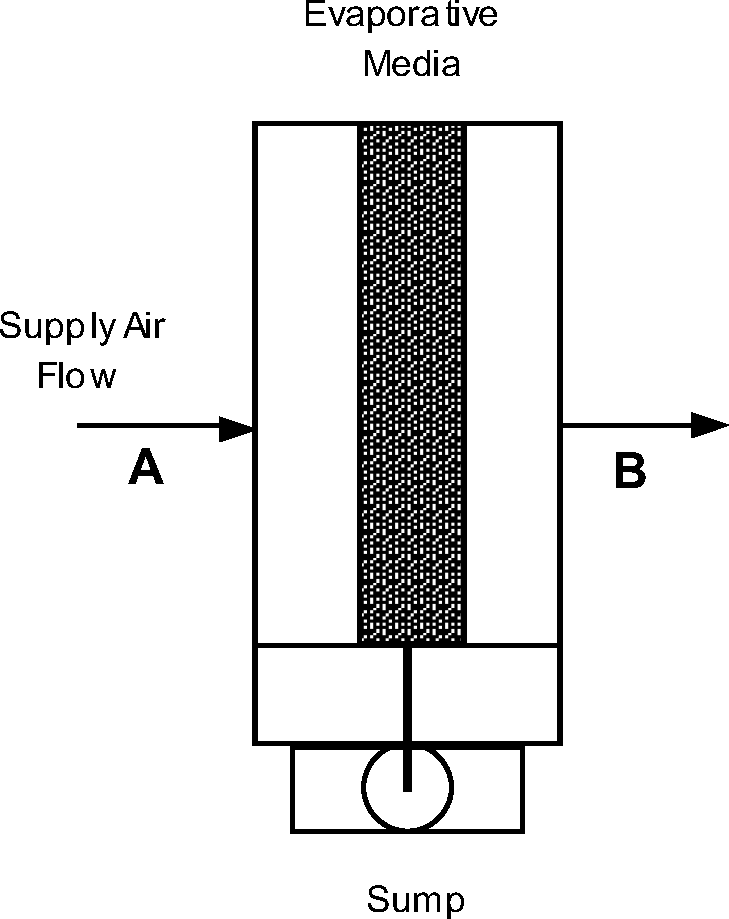
\includegraphics[width=0.9\textwidth, height=0.9\textheight, keepaspectratio=true]{media/image4789.png}
\caption{Direct Stage Evaporative Cooler \protect \label{fig:direct-stage-evaporative-cooler}}
\end{figure}

The thermodynamic process is a simultaneous heat and mass transfer, or adiabatic cooling, and follows a constant enthalpy line on the psychrometric chart; it is shown in the figure below as a process from A to B.~ Since the deviation of the constant wet-bulb line and the constant enthalpy line is small, it is assumed that the wet-bulb temperature is constant across the direct evaporative stage.

\begin{figure}[hbtp] % fig 198
\centering
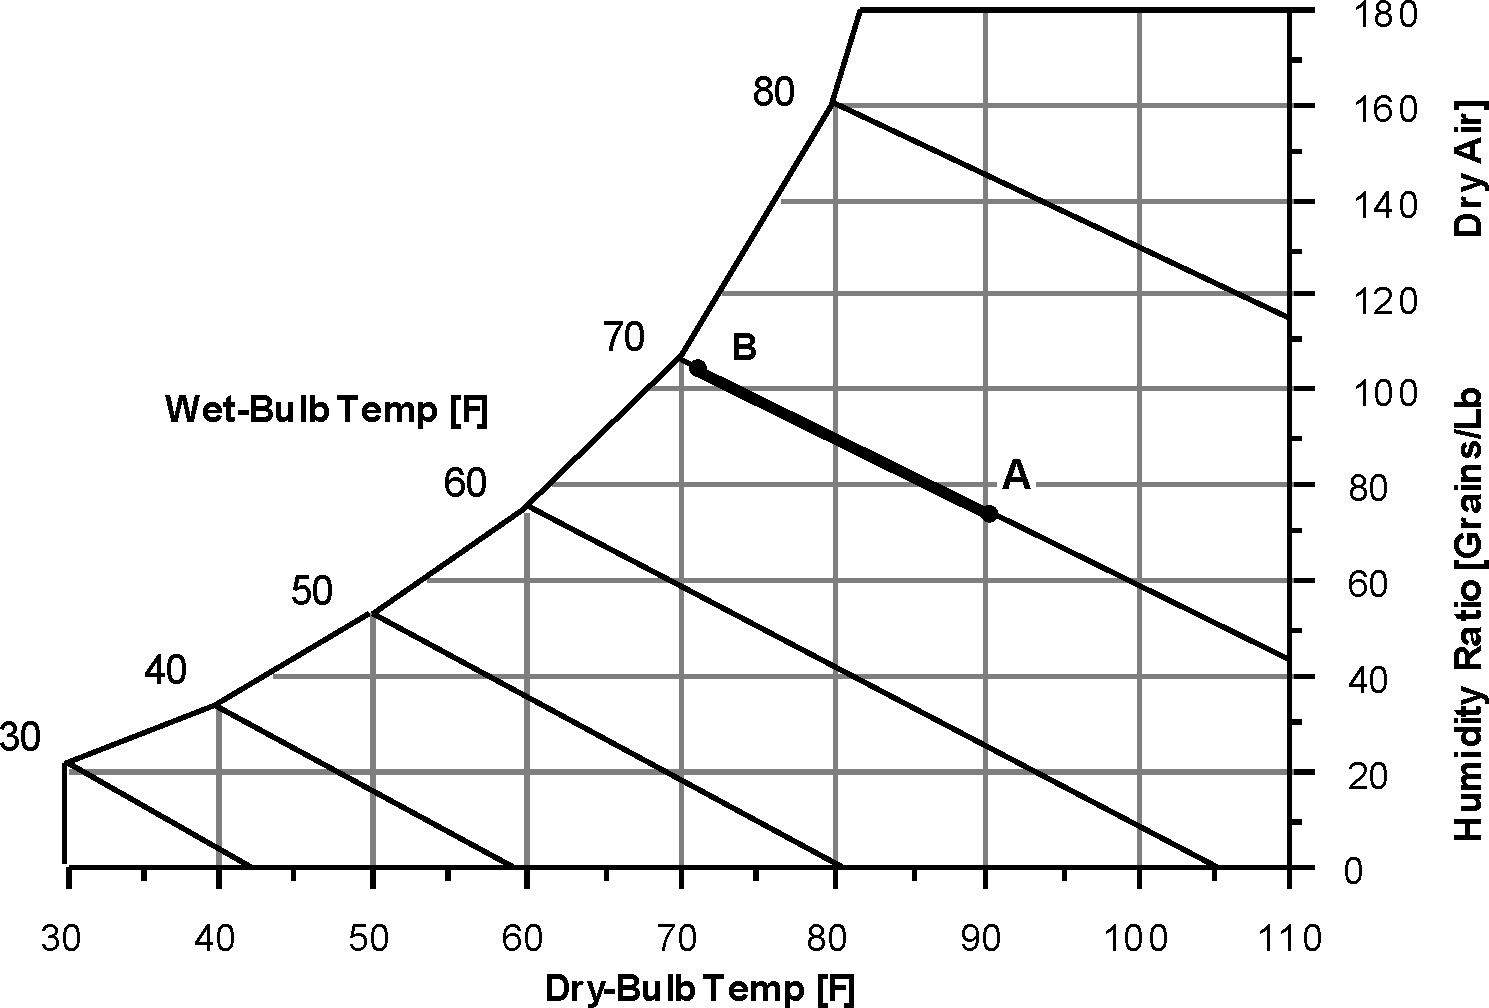
\includegraphics[width=0.9\textwidth, height=0.9\textheight, keepaspectratio=true]{media/image4790.png}
\caption{Psychrometric Chart -- Constant Enthalpy \protect \label{fig:psychrometric-chart-constant-enthalpy}}
\end{figure}

If the direct evaporative process were 100\% efficient, the leaving dry-bulb temperature would equal the entering wet-bulb temperature.~ The efficiency of the direct evaporative process is less than 100\% and by defining saturation efficiency (ese) for the direct stage or evaporative pad, the leaving dry-bulb temperature can be expressed by the following equation.

\begin{equation}
{T_{dbsupout}} - {T_{dbsupin}} = {\varepsilon_{se}} \cdot \left( {{T_{odb}} - {T_{owb}}} \right)
\end{equation}

\subsubsection{Saturation Efficiency}\label{saturation-efficiency}

Since the evaporative process is not 100\% efficient the saturation efficiency is defined by.

\begin{equation}
{\varepsilon_{se}} = \frac{{{T_{dbsupin}} - {T_{dbsupout}}}}{{{T_{odb}} - {T_{owb}}}}
\end{equation}

The saturation efficiency is determined from manufacturer's data, and the least squares curve fit is discussed in Curve Fitting Evaporative Media section.

Using the saturation efficiency (ese) for the direct stage evaporative pad, the leaving dry-bulb temperature can be determined directly.~ The evaporative process approximately follows a constant wet-bulb line.~ Therefore, with the leaving dry-bulb temperature and assuming adiabatic heat transfer across the direct stage, the outlet conditions for the direct stage are known.

The saturation efficiency of the direct evaporative cooler is a function of the pad geometry and airflow rate.~ The pad geometry is constant throughout the simulation, but the airflow rate can change from hour to hour when the evaporative cooler is used with an air economizer.~ The saturation efficiency would then be determined from the flow for that hour with the geometry of the direct evaporative cooler.~ This gives the dry-bulb temperature leaving the evaporative cooler.~ Assuming adiabatic heat transfer across the direct stage, the evaporative process follows the constant wet-bulb line or the constant enthalpy line on the psychrometric chart, therefore the wet-bulb temperature is constant from inlet to outlet.

Some things that can cause departure from the ideal adiabatic saturation process in the direct evaporative cooler are:

·~~~~~~~~makeup water entering the sump,

·~~~~~~~~friction from water re-circulation,

·~~~~~~~~heat transfer from surroundings,

·~~~~~~~~solar radiation (sun upon a cooler).

Thus, adiabatic saturation in evaporative cooling is only an approximation, however the adiabatic saturation assumption in the rigid-media cooler is good, since the water recirculates rapidly and approximates the wet-bulb temperature at steady state operation.

\subsubsection{Curve Fitting Evaporative Media}\label{curve-fitting-evaporative-media}

The saturation efficiency is usually reported as a function of airflow, pad face velocity, and pad thickness.~ The Figure below shows a typical graph of manufacturer's data for the saturation efficiency.~ A multi-variate least squares curve fit of the data was used to generate saturation efficiency functions for the evaporative models that use the CelDek rigid media pad.

\begin{figure}[hbtp] % fig 199
\centering
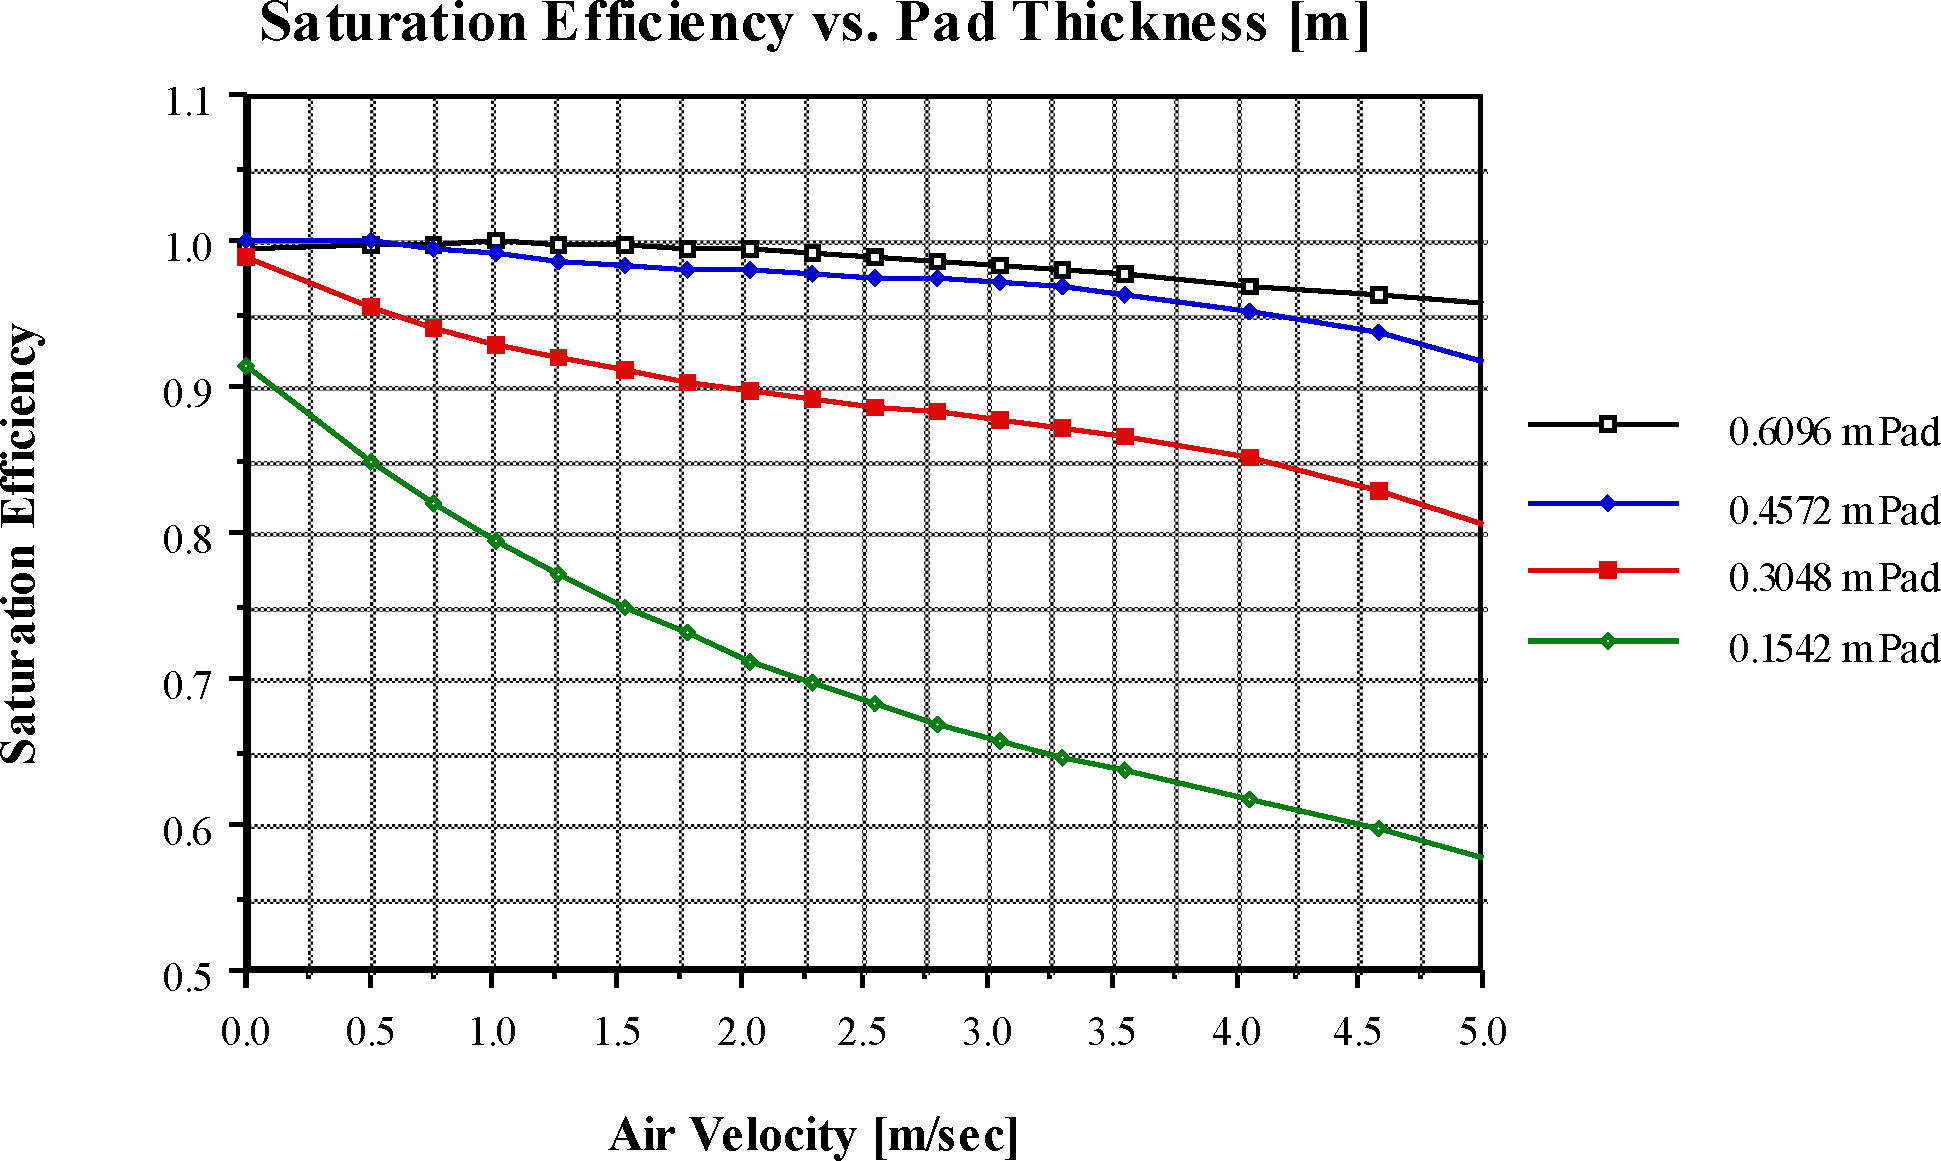
\includegraphics[width=0.9\textwidth, height=0.9\textheight, keepaspectratio=true]{media/image4793.png}
\caption{Graph of Saturation Efficiency \protect \label{fig:graph-of-saturation-efficiency}}
\end{figure}

The curve fit for saturation efficiency was obtained using the functions listed below.~ The model uses the air velocity (Airvel) through the pad and the depth of the media (Depth).~ The least squares routine produced the following model that is used for the evaporative cooling rigid media pad.~ The least squares routine produced an eleven-term multi-variate fit using a third order quadratic.

ese~ = 0.792714 + 0.958569 (Depth) - 0.25193 (Airvel) - 1.03215 (Depth\(^{2}\)) + 0.0262659~(Airvel\(^{2}\)) + 0.914869 (Depth * Airvel) - 1.48241 (Airvel * Depth\(^{2}\)) - 0.018992 (Airvel\(^{3}\) * Depth) + 1.13137 (Depth\(^{3}\) * Airvel) + 0.0327622~(Airvel\(^{3}\) * Depth\(^{2}\)) - 0.145384 (Depth\(^{3}\) * Airvel\(^{2}\))

Where Airvel is in meters per second and Depth is in meters.~ This curve fit is used for the rigid media in the EvapCooler:Direct:CelDekPad and EvapCooler:InDirect:CelDekPad.

\subsection{Dry Coil Indirect Evaporative Cooler}\label{dry-coil-indirect-evaporative-cooler}

The input object EvaporativeCooler:Indirect:CelDekPad provides a model of a dry coil indirect evaporative cooler, shown in the figure below, that has a rigid media pad, similar to the direct evaporative stage, where the adiabatic cooling takes place.~ The secondary air leaves the rigid media pad and enters an air-to-air heat exchanger where it cools the supply air flowing through the heat exchanger tubes.~ The moist secondary air is then exhausted to the environment.~ The secondary air stream has its own fan and includes consists of a rigid media evaporative pad, with water recirculated from a reservoir.~ The water is pumped from the reservoir to a water distribution header, for water feed by gravity from above the media.~ The evaporative pad provides the area for the adiabatic saturation of the air.

\begin{figure}[hbtp] % fig 200
\centering
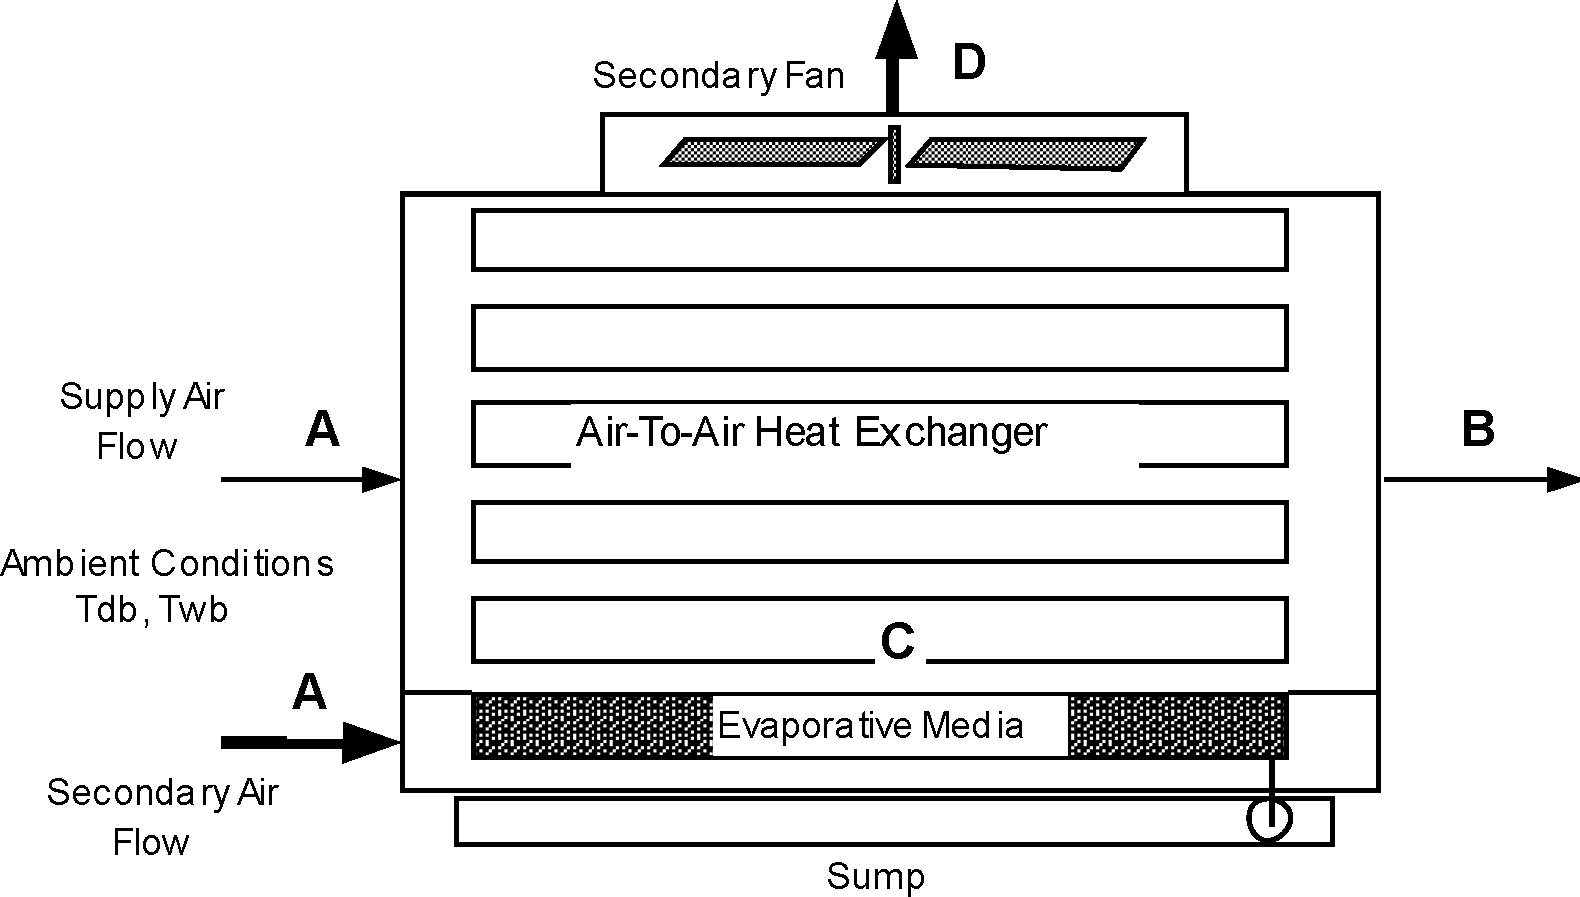
\includegraphics[width=0.9\textwidth, height=0.9\textheight, keepaspectratio=true]{media/image4794.png}
\caption{Evaporative Cooler -- Indirect Dry Coil \protect \label{fig:evaporative-cooler-indirect-dry-coil}}
\end{figure}

The process that the secondary air goes through, A to C to D, is shown by the dashed lines in~ the following figure.~ Process A to C is adiabatic cooling in the rigid media pad.~ Then the air enters the shell side of the heat exchanger and is sensibly heated from C to D by the warm supply air passing through the tube side.

\begin{figure}[hbtp] % fig 201
\centering
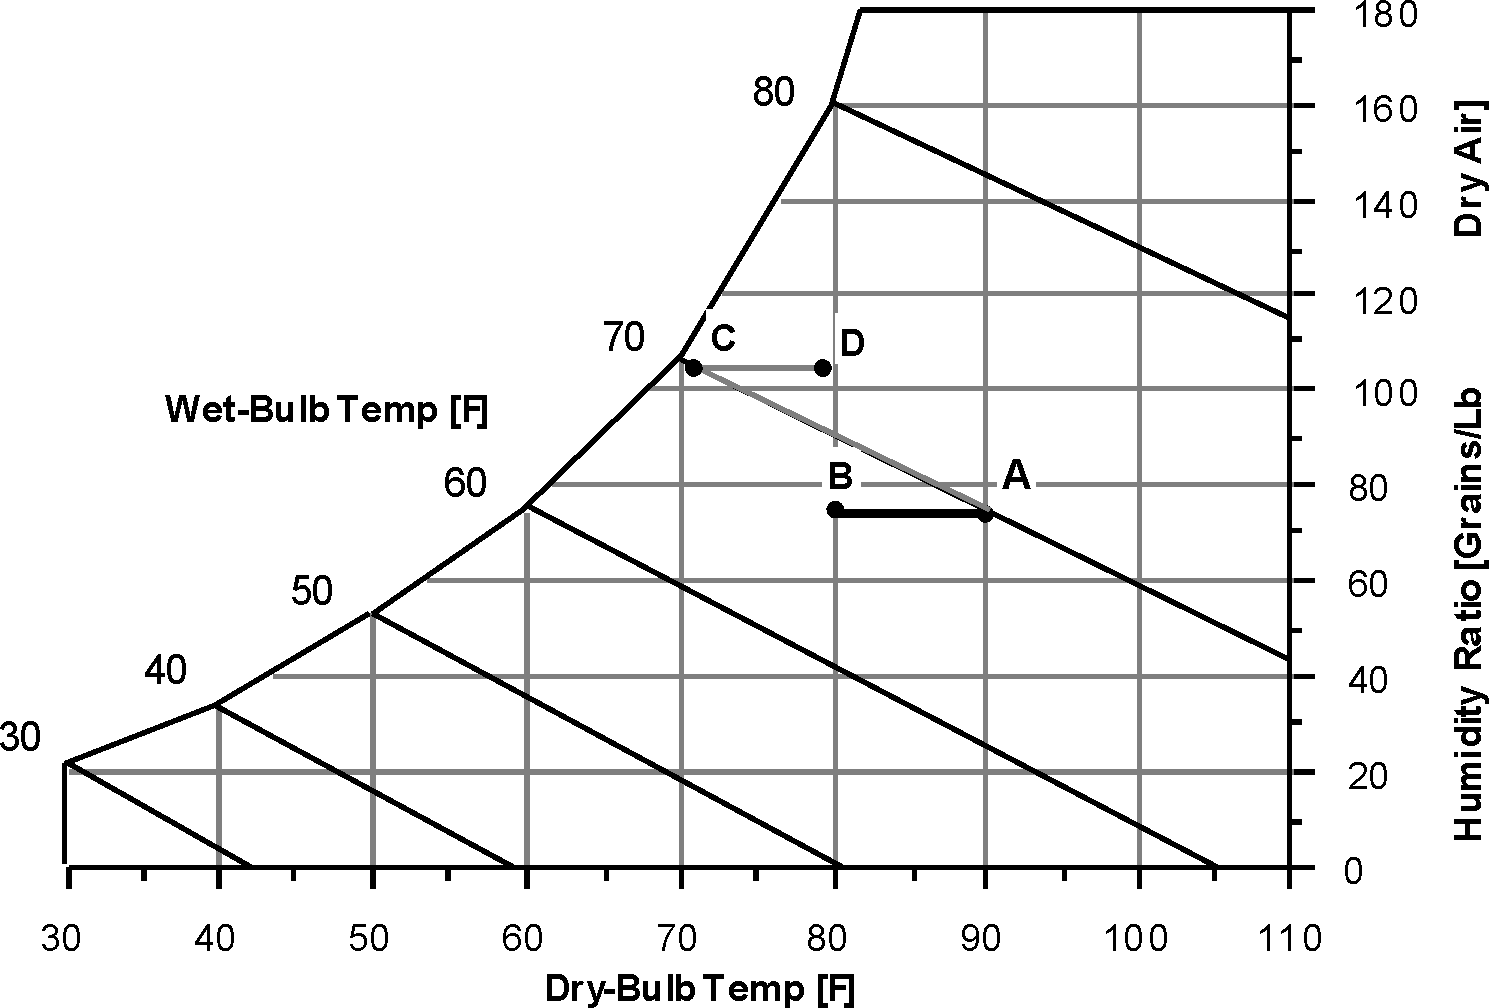
\includegraphics[width=0.9\textwidth, height=0.9\textheight, keepaspectratio=true]{media/image4795.png}
\caption{Secondary Air Process -- Indirect Dry Coil Evap Cooler \protect \label{fig:secondary-air-process-indirect-dry-coil-evap}}
\end{figure}

The advantage of the dry coil heat exchanger is that the heat exchanger does not have the evaporation taking place on the outside of the tubes, thus no mineral deposits are left on the heat exchange surface to reduce the efficiency of the heat exchanger.~ The rigid media pads are designed to flush the mineral deposits to the sump, so the saturation efficiency of the pad stays relatively constant.

The following equations are used to determine the dry-bulb temperature leaving the evaporative media, given pad geometry and secondary airflow information.~ The heat transfer in the heat exchanger can be determined with the effectiveness of the heat exchanger according.

Tdb sup out = Tdb sup in - ese*(Todb - Towb )

QHx~ = eHx~* Min( CFMsec~, CFMsupply) * rair~* cp air~* ( Todb~- Tdb sec out)

After the heat transfer for the heat exchanger has been determined, an energy balance is done on the supply airside to determine the dry-bulb temperature leaving the indirect evaporative cooler. ~This assumes all the energy for is provided by the primary air stream so the effectiveness value includes the air-to-air effectiveness of the heat exchanger.

Tdb sup out = ~ Tdb sup in~~ -~ \(\frac{{{Q_{Hx}}}}{{{r_{air}}*{c_{pair}}*CF{M_{\sup ply}}}}\)

The wet-bulb temperature is determined from psychrometric routines using the leaving dry-bulb temperature, humidity ratio, and barometric pressure, since humidity ratio is constant for the supply air across the indirect stage.~ The effectiveness of the heat exchanger is determined from a parameter estimation using manufacturer's performance data.~ For the indirect evaporative cooler it was found that a value of 0.67 represented reasonable default effectiveness.

\subsection{Wet Coil Indirect Evaporative Cooler}\label{wet-coil-indirect-evaporative-cooler}

The input object EvaporativeCooler:Indirect:WetCoil provides a model for a wetted coil evaporative cooler, shown in the figure below, that has water sprayed directly on the tubes of the heat exchanger where latent cooling takes place.~ The vaporization of the water on the outside of the heat exchanger tubes allows the simultaneous heat and mass transfer which removes heat from the supply air on the tube side.~ Then the moist secondary air is exhausted.~ The secondary air stream has its own fan.

\begin{figure}[hbtp] % fig 202
\centering
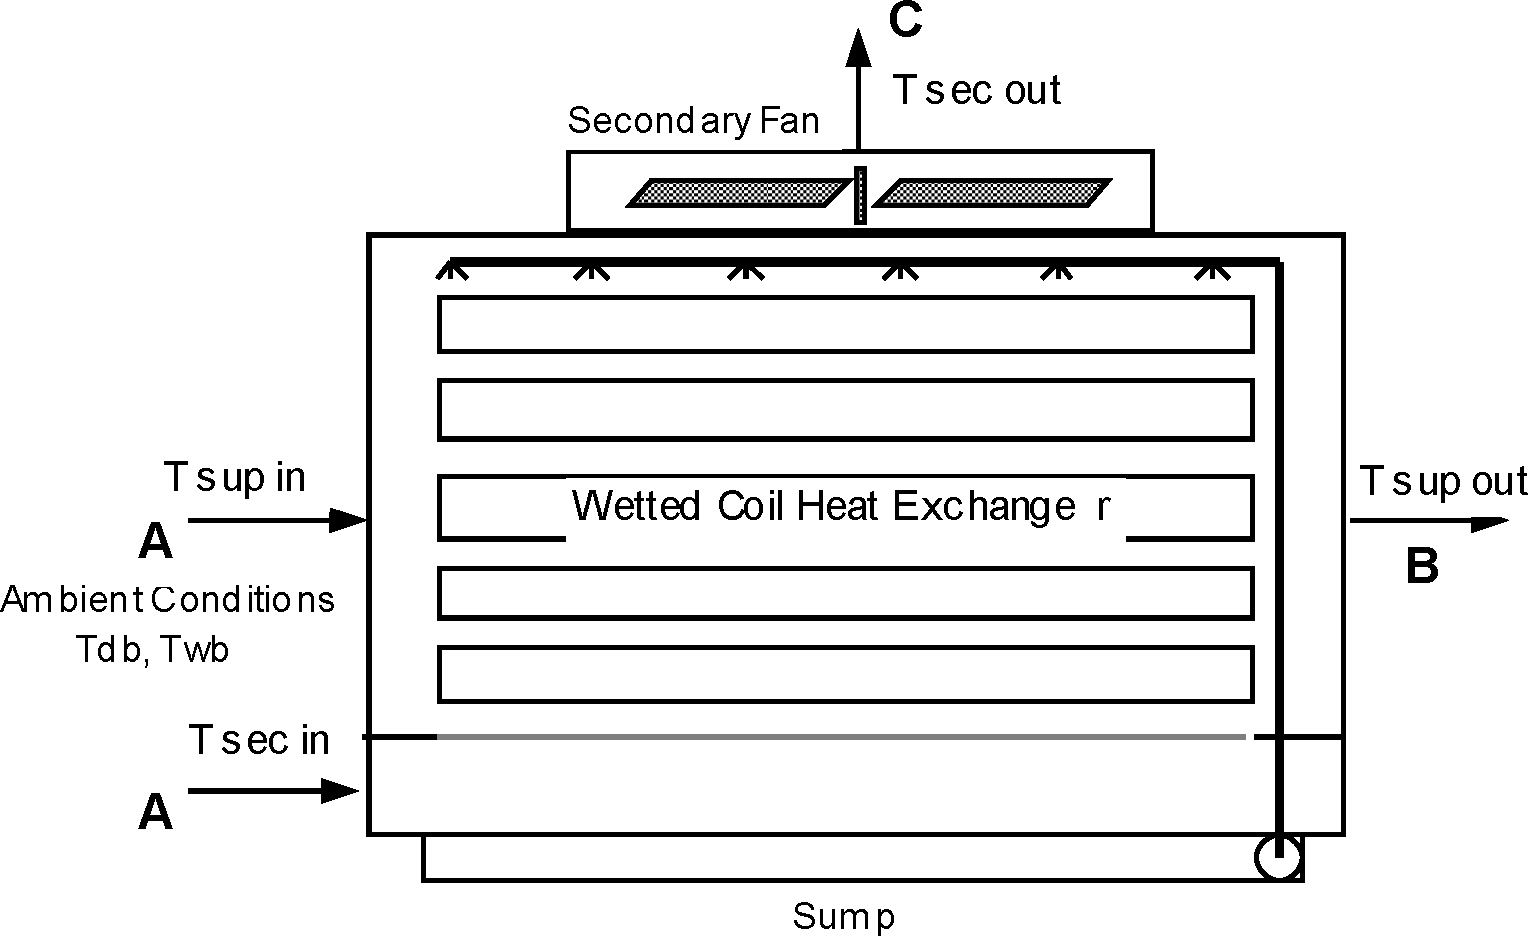
\includegraphics[width=0.9\textwidth, height=0.9\textheight, keepaspectratio=true]{media/image4797.png}
\caption{Wet Coil Indirect Evaporative Cooler \protect \label{fig:wet-coil-indirect-evaporative-cooler}}
\end{figure}

The process that the secondary air goes through, A to C on the following figure, is a path of simultaneous heat and mass transfer, but it does not follow a line of constant enthalpy as in the direct stage.~ The process is not adiabatic due to the heat gain from the supply air flowing through the tubes of the heat exchanger.

\begin{figure}[hbtp] % fig 203
\centering
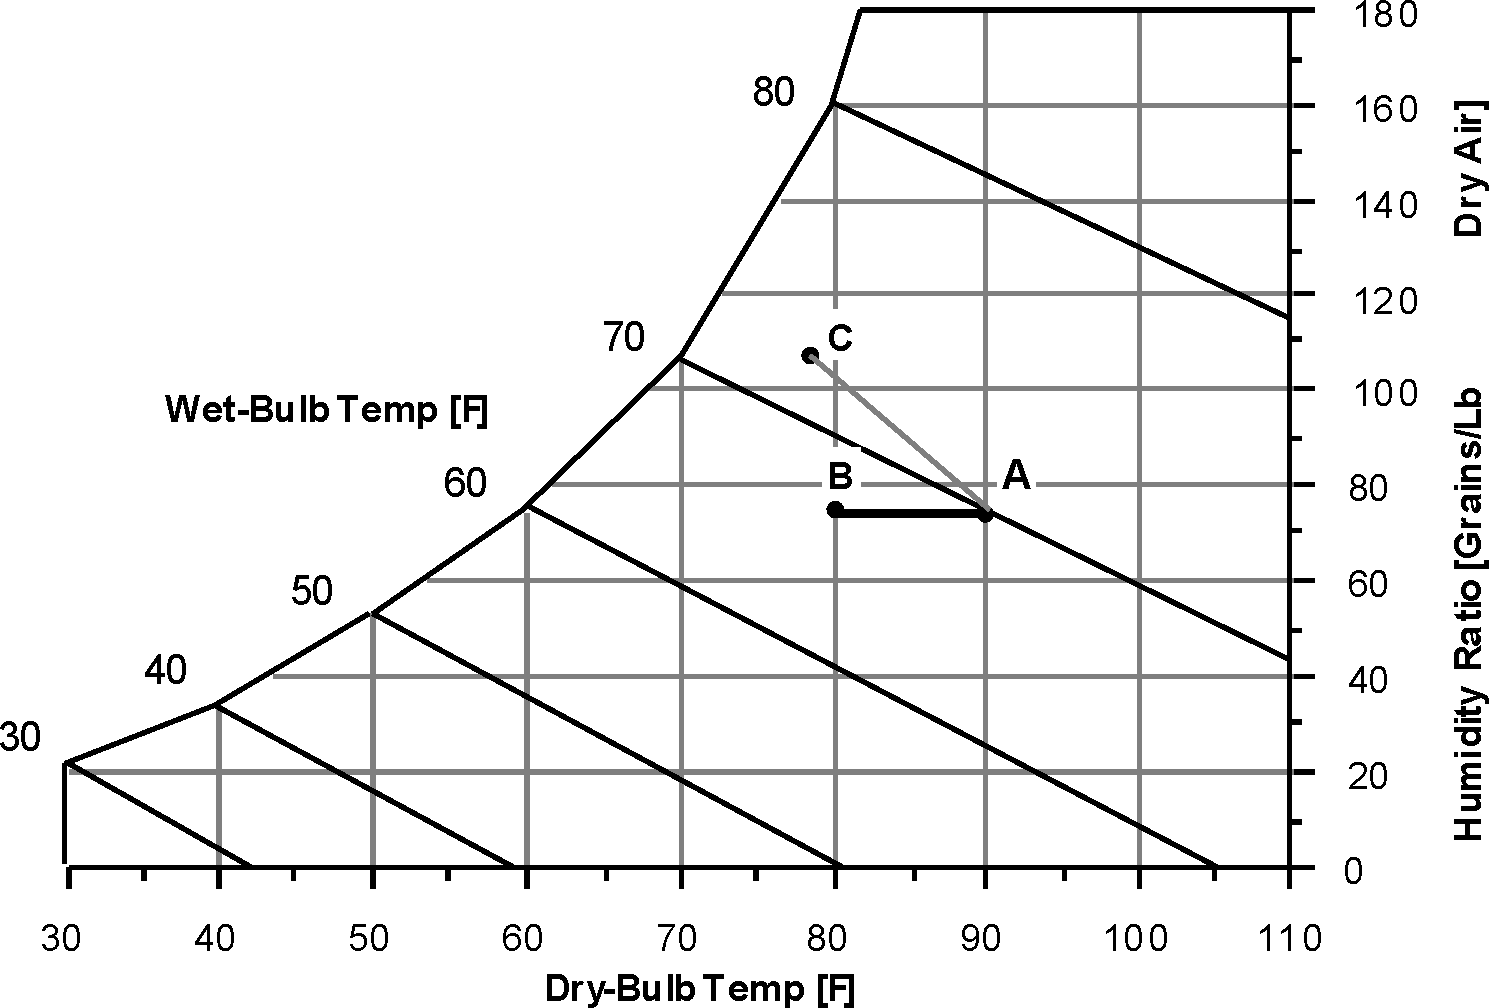
\includegraphics[width=0.9\textwidth, height=0.9\textheight, keepaspectratio=true]{media/image4798.png}
\caption{Secondary Air Process – Indirect Wet Coil Evaporative Cooler \protect \label{fig:secondary-air-process-indirect-wet-coil}}
\end{figure}

The wet coil heat exchanger can have a higher stage efficiency than the dry coil due to a higher heat transfer rate on the outside of the heat exchanger tubes.~ Over the operating lifetime of the heat exchanger, the vaporization taking place on the heat exchange surface can leave mineral deposits that will decrease the effectiveness of the heat exchanger.

\subsubsection{Efficiencies of the Indirect Stage}\label{efficiencies-of-the-indirect-stage}

In an indirect stage of an evaporative cooler, the secondary or wet side air stream acts as a heat sink for the supply air.~ The efficiency of the indirect stage is given as the effectiveness of the sensible heat exchange, eHx, and the saturation efficiency on the wet streamside, ese.~ These are expressed as:

eHx~ = \(\frac{q}{{{q_{max}}}}\) = ~ \(\frac{{{C_{sup}}({T_{supin}} - {T_{supout}})}}{{{C_{min}}({T_{secin}} - {T_{secout}})}}\) ,

ese~ = ~ \(\frac{{{T_{dbsecin}} - {T_{dbsecout}}}}{{{T_{odb}} - {T_{owb}}}}\) ,

where Tdb sup in~ = Tdb sec in~ for the indirect cooler.~ The maximum heat transfer possible would be obtained if the supply stream was cooled all the way to the wet-bulb temperature.~ So the efficiency of the indirect evaporative cooler is defined by:

eind~ = ~ \(\frac{{({T_{dbsupin}} - {T_{dbsupout}})}}{{({T_{odb}} - {T_{owb}})}}\) .

Using the combination of the effectiveness and saturation efficiency, the total efficiency of the indirect stage can be expressed by:

eind~ = eHx~ ese~ \(\frac{{{C_{sup}}}}{{{C_{min}}}}\) .

In many cases Csup = Cmin and the efficiency of the indirect stage reduces to:

eind~ = eHx~ ese.

An intuitive model determining the performance of the wet coil indirect model was developed.~ This model can be used for all indirect models by curve fitting data from the evaporative cooler of interest.~ The model development starts with the total efficiency of the indirect evaporative cooler:

eind~ = ~ \(\frac{{({T_{dbsupin}} - {T_{dbsupout}})}}{{({T_{odb}} - {T_{owb}})}}\)

Solving for T db sup out~gives the leaving conditions of the supply air at a constant humidity ratio:

T db sup out = Tdb sup in - eind * (Todb - Towb)

A form for the efficiency of the indirect stage was devised using a maximum efficiency with a coefficient to reduce the efficiency depending on the ratio of the airflows.

eind~ = emax~- C1~* (\(\frac{{CF{M_{sup}}}}{{CF{M_{sec}}}}\) )

C1~is the ``Flow Efficiency Ratio'' and is determined from performance data.

A check of limits will verify that it makes physical sense.~ As the magnitude of the secondary flow increases, the second term of equation above becomes smaller.~ This would make the efficiency tend to go to the maximum efficiency.~ Physically this would be true since the convective terms for heat and mass transfer would increase on the outside of the tube with the additional mass flow rate.~ Similarly, if the supply air flow goes to zero with a constant secondary air flow, the second term of the equation above again becomes small, and the overall efficiency of the stage would approach the maximum.~ The constant C1~tells how quickly the efficiency of the stage would decrease with a mismatch of the supply and secondary flows.

The maximum efficiency of the stage is a combination of the efficiency due to the simultaneous heat and mass transfer on the outside of the tube and the efficiency of the heat exchanger.~ This value can be higher than the dry coil overall efficiency since the convective coefficients on the outside of the tube are larger.~ For example, a least squares fit for the maximum efficiency showed this value was approximately 0.8 compared to the dry coil indirect value of approximately 0.65 (0.67 * 0.97).~ (The maximum efficiency for the dry coil indirect was determined at the condition where flow through the evaporative pad in the secondary air stream approached zero, for a 12-inch thick pad.)~ It should be noted again that over the operating life of the wet coil heat exchanger, the mineral deposits that are left can decrease the effectiveness of the heat exchanger unless appropriate maintenance has taken place.~ Therefore, if modeling an older system, the manufacturer's data may no longer describe the equipment effectiveness.

\subsection{Two Stage Direct/Indirect Evaporative Cooler}\label{two-stage-directindirect-evaporative-cooler}

A two stage cooler can be modeled by combining either a wet coil or the dry coil indirect evaporative cooler staged with a direct evaporative cooler.~ The figure below shows a dry coil indirect evaporative cooler with a direct evaporative cooler.~ This configuration is mainly used for total comfort cooling for a building and would not normally be used as a pre-cooler for a refrigeration coil, since the direct stage would increase the latent load on a refrigeration coil.

\begin{figure}[hbtp] % fig 204
\centering
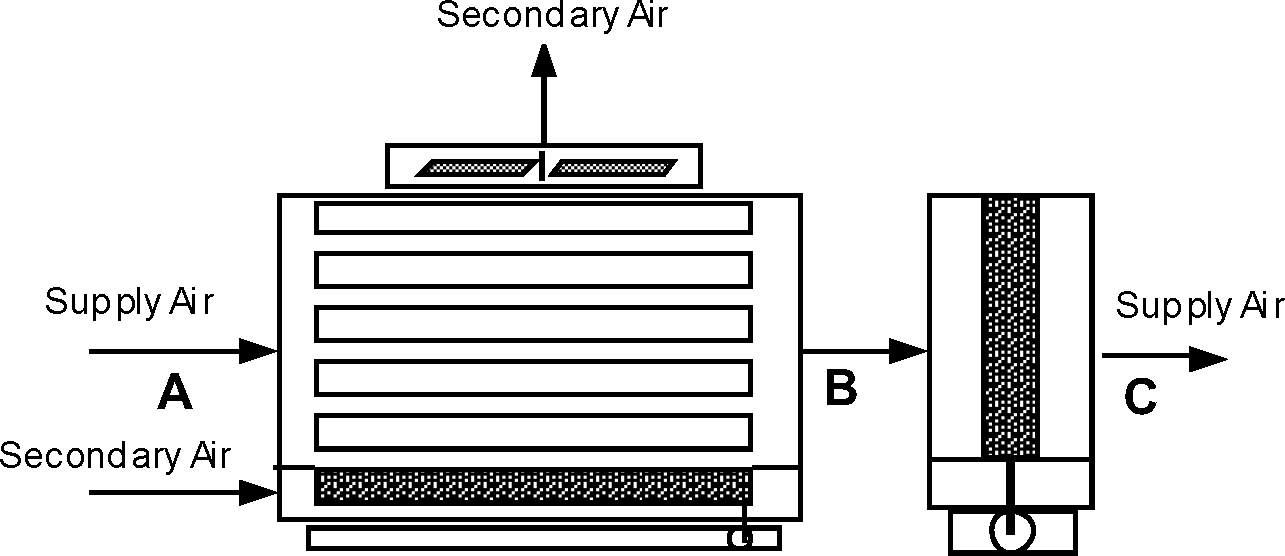
\includegraphics[width=0.9\textwidth, height=0.9\textheight, keepaspectratio=true]{media/image4806.png}
\caption{Two Stage Evaporative Cooler \protect \label{fig:two-stage-evaporative-cooler}}
\end{figure}

The thermodynamic process for the supply air is shown below, going from A to B to C.~ The process from A to B is sensible cooling in the indirect stage.~ The process from B to C is simultaneous heat and mass transfer following a constant enthalpy line.~ The air leaving the final stage has a lower dry-bulb and wet-bulb temperature, and an increase in moisture from the direct stage.

\begin{figure}[hbtp] % fig 205
\centering
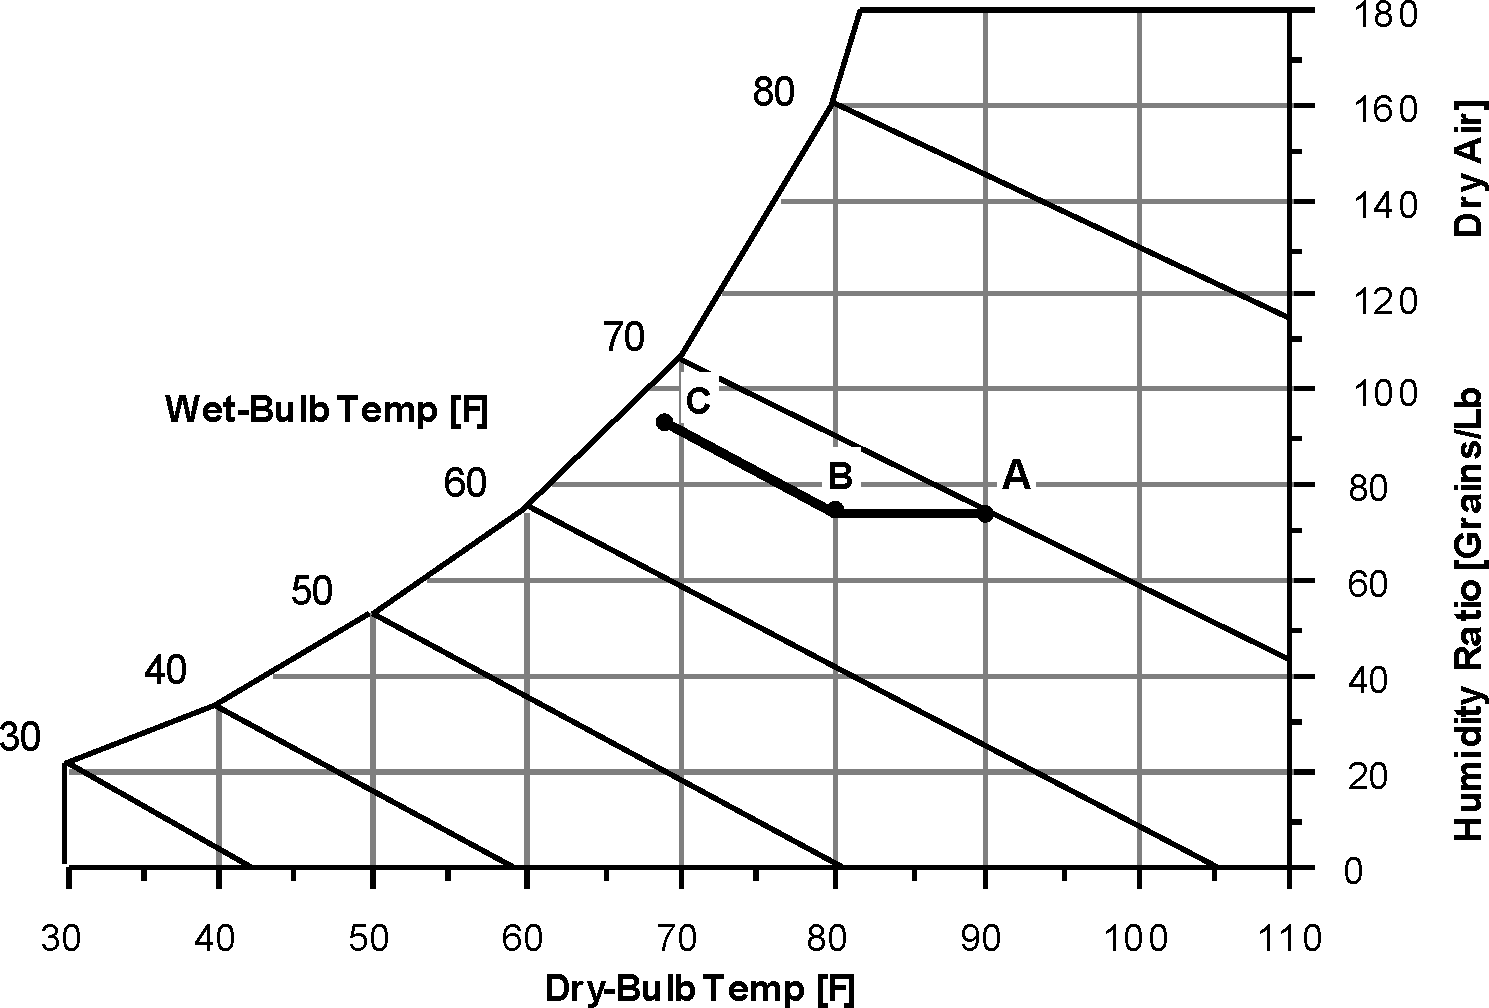
\includegraphics[width=0.9\textwidth, height=0.9\textheight, keepaspectratio=true]{media/image4807.png}
\caption{Thermodynamic Process for Supply Air Through Two Stage Evaporative Cooler \protect \label{fig:thermodynamic-process-for-supply-air-through}}
\end{figure}

Two stage evaporative coolers can be accomplished by putting the EvaporativeCooler:Direct:CelDekPad, EvaporativeCooler:Indirect:CelDekPad, EvaporativeCooler:Indirect:WetCoil in series in any combination the user desires in the supply air loop.

\subsection{Indirect Evaporative Cooler Special Research Model}\label{indirect-evaporative-cooler-special-research-model}

This section summarizes the model implemented in the component EvaporativeCooler:Indirect:ResearchSpecial.~ Examples of this evaporative cooler are shown in the following figures, without and with a relief valve. This model differs from the other indirect evaporative coolers in that, under part load conditions, it can modulate so that the air leaving the cooler just meets a drybulb temperature setpoint.

The indirect research special evaporative cooler (IEC) machine provides improved modeling features needed for data center and other hybrid cooling applications. The new model includes performance curves for variable effectiveness, fan power, and pump power. It is intended to be able to model IEC machines that have 1) variable speed secondary fans, 2) variable speed pumps for water recirculation and spraying, and 3) ability to operate in a dry mode. Such IEC machines can modulate the cooling power during operation by varying either the secondary side fan speed or the intensity of water spray or both. To simplify the model it is assumed that the device's internal controls are such that, when it is operating as a ``Wet'' evaporative cooler, secondary fan and spray pump operation are linked together so that there is a one-to-one mapping between them at any given part load situation. This allows formulating the fan and pump power performance curves to be based on the same independent variable, secondary air flow fraction.

\begin{figure}[hbtp] % fig 206
\centering
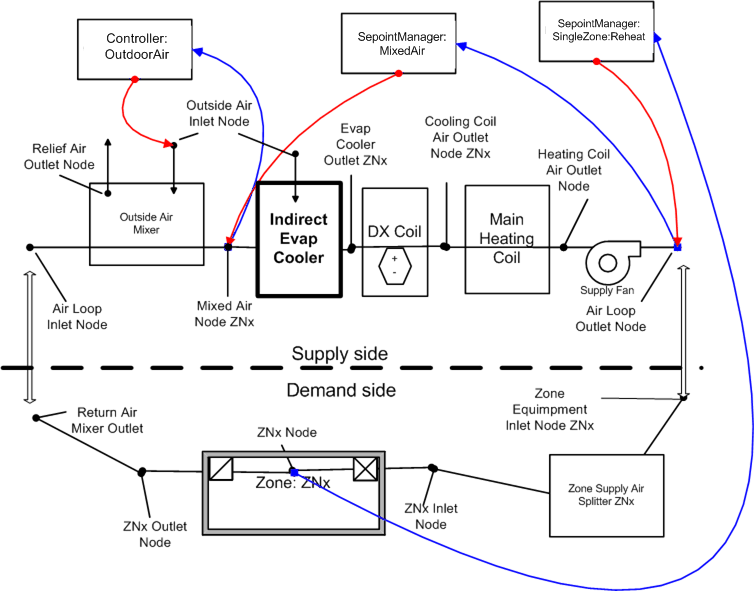
\includegraphics[width=0.9\textwidth, height=0.9\textheight, keepaspectratio=true]{media/image4808.png}
\caption{Research Special Indirect Evaporative Cooler \protect \label{fig:research-special-indirect-evaporative-cooler}}
\end{figure}

\subsubsection{Model Formulation}\label{model-formulation}

Each time the model is called it takes the inputs on the left and produces the outputs on the right as shown in \protect\hyperlink{IndEvapCoolerFig2}{Figure}. ``sys'' is primary air stream and typically sits on an AirLoop HVAC branch. ``sec'' is secondary purge air stream and is typically outdoor air. The model will set node flow rates and ``out\_sec'' state variables on the secondary outlet.

\begin{figure}[htbp]
\centering
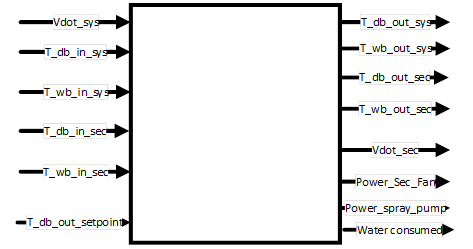
\includegraphics{media/image8005.png}
\caption{}
\end{figure}

Figure: Illustration of Inputs-Outputs of Indirect Evaporative Cooler Research Special

The model runs either in dry mode or wet mode depending entering air conditions of the primary and secondary air sides. Different effectiveness values are used depending on the operating modes.

\subsubsection{Wet Mode Operation}\label{wet-mode-operation}

If running ``wet,'' use wet bulb effectiveness and wet bulb temperature depression for delta T:

\begin{equation}
\begin{array}{rl}
  \epsilon_{wb,op} & = \epsilon_{wb,design}\cdot f_{wb,mod}\left(\text{flowRatio}\right) \\
  \text{flowRatio} & = \frac{\dot{m}_{sec}}{\dot{m}_{sys}}
\end{array}
\end{equation}

Where:

\begin{itemize}
\item
  \(\epsilon_{wb,op}\) = current operation effectiveness with respect to wet bulb temperature depression.
\item
  \(\epsilon_{wb,design}\) = user input for effectiveness at design air flow rates and full spray power
\item
  \(f_{wb,mod}\) = normalized wet mode operation effectiveness modifier performance curve as a function of flow fraction. The curve value describes how effectiveness varies at different flow rates. When conditions are appropriate, this curve is numerically inverted to find a FlowRatio that just meets a setpoint.
\item
  \(\dot{m}_{sys}\) = primary air current time step mass flow rate in kg/s
\item
  \(\dot{m}_{sec}\) = secondary air current time step mass flow rate in kg/s
\end{itemize}

The leaving primary air dry bulb temperature in wet operating mode is calculated as follows:

\begin{equation}
T_{db,out,sys} = T_{db,in,sys} - \epsilon_{wb,op} \left( T_{db,in,sys} - T_{wb,in,sec} \right)
\end{equation}

Then check that there is sufficient heat capacitance flux (mcT) in the secondary air stream to provide the conditioning. The following steps are for checking and adjusting for non-physical outcomes that could happen with low secondary flow rates.

\begin{enumerate}
\def\labelenumi{\arabic{enumi}.}
\tightlist
\item
  Calculate heat transfer rate
\end{enumerate}

The secondary air entering wet-bulb temperature would be the loswest limit allowed, although this temperature cannot be attained in most practical situations. This is checked as a limiting case.

\begin{equation}
  \begin{array}{rl}
    T_{db,out,sys} & = \max\left(T_{db,out,sys},T_{db,out,setpoint}\right) \\
    \dot{Q}_{HX} & = \left(\dot{m}c_p\right)_{sys,in} \cdot \left(T_{db,in,sys}-T_{db,out,sys}\right)
  \end{array}
\end{equation}

\begin{enumerate}
\def\labelenumi{\arabic{enumi}.}
\setcounter{enumi}{1}
\tightlist
\item
  Calculate outlet enthalpy of the secondary air
\end{enumerate}

\begin{equation}
\text{enahalpy}_{out,sec} = \text{enthalpy}_{in,sec} + \frac{\dot{Q}_{HX}}{\dot{m}_{sec}}
\end{equation}

One approximation that can be made is the outlet condition of the temperature and humidity ratio combination that produces the outlet enthalpy of the secondary air calculated above. A conservative approach is that the secondary air leaves with water added at such a rate that it results in the secondary air to leave at the same dry bulb temperature and all the total heat transfer results in humidity ratio increases, i.e., latent heat transfer. Following this assumption the secondary air outlet humidity ratio can be calculated in step 3.

\begin{enumerate}
\def\labelenumi{\arabic{enumi}.}
\setcounter{enumi}{2}
\tightlist
\item
  Calculate outlet humidity ratio of the secondary air
\end{enumerate}

\begin{equation}
  \begin{array}{rl}
    T_{db,out,sec} & = T_{db,in,sec} \\
    \text{HumRat}_{out,sec} & = \text{PsyWFnTbH}\left(T_{db,out,sec},\text{enthalpy}_{out,sec}\right) \\
    \dot{V}_{water} & = \frac{QHX / \left[ \left(\text{HumRat}_{out,sec}-\text{HumRat}_{in,sec}\right) \cdot h_{fg,in,sec}\right]}{\rho_{water,Tdb,in,sec}} \\
    or & = \\
    \dot{V}_{water} & = \frac{QHX / \left[ \left(\text{enthalpy}_{out,sec}-\text{enthalpy}_{in,sec}\right) \right]}{\rho_{water,Tdb,in,sec}}
  \end{array}
\end{equation}

Dry Operation Mode

Similarly, if running ``dry'' use dry bulb effectiveness and dry bulb based delta T

\begin{equation}
\epsilon_{db,op} = \epsilon_{db,design} \cdot f_{db,mod}\left(\text{flowRatio}\right)
\end{equation}

Where:

\begin{itemize}
\item
  \(\epsilon_{db,op}\) = current operation effectiveness with respect to dry bulb temperature depression.
\item
  \(\epsilon_{db,design}\) = user input for effectiveness at design air flow rates and dry operation mode (no water spray on the secondary air side)
\item
  \(f_{db,mod}\) = normalized dry mode operation effectiveness modifier performance curve as a function of flow fraction. The curve value describes how the dry mode effectiveness varies with different flow rates. When conditions are appropriate, this curve is numerically inverted to find a FlowRatio that just meets a setpoint
\end{itemize}

The leaving primary air dry bulb temperature in dry operating mode is calculated as follows:

\begin{equation}
T_{db,out,sys} = T_{db,in,sys} - \epsilon{db,op}\left(T_{db,in,sys}-T_{db,in,sec}\right)
\end{equation}

Then check that there is sufficient heat capacitance flux (mcT) in the secondary air stream to provide the conditioning. For dry operation, it should be sufficient to simply use inlet moist air properties for density and specific heat. The following steps are for checking and adjusting for non-physical outcomes that could happen with low secondary flow rates.

\begin{enumerate}
\def\labelenumi{\arabic{enumi}.}
\tightlist
\item
  Calculate heat transfer
\end{enumerate}

\begin{equation}
\dot{Q}_{HX} = \left(\dot{m}c_{p}\right)_{sys,in} \left(T_{db,in,sys}-T_{db,out,sys}c\right)
\end{equation}

\begin{enumerate}
\def\labelenumi{\arabic{enumi}.}
\setcounter{enumi}{1}
\tightlist
\item
  Calculate secondary/scavenger leaving dry-bulb
\end{enumerate}

\begin{equation}
T_{db,out,sec} = T_{db,in,sec} + \frac{\dot{Q}_{HX}}{ \left(\dot{m}c_{p}\right)_{sys,in}}
\end{equation}

\begin{enumerate}
\def\labelenumi{\arabic{enumi}.}
\setcounter{enumi}{2}
\tightlist
\item
  Check for energy imbalance and adjust if need
\end{enumerate}

\begin{equation}
\text{IF} \left(T_{db,out,sec}>T_{db,in,sys}\right) \text{THEN} T_{db,out,sec} = T_{db,in,sys}-0.2 C
\end{equation}

\begin{enumerate}
\def\labelenumi{\arabic{enumi}.}
\setcounter{enumi}{3}
\tightlist
\item
  Recalculate heat transfer limit if imbalance found in step 3 using new secondary outlet drybulb
\end{enumerate}

\begin{equation}
\dot{Q}_{HX,lim} = \left(\dot{m}c_{p}\right)_{sec,in}\cdot \left( T_{db,out,sec}-T_{db,in,sec} \right)
\end{equation}

\begin{enumerate}
\def\labelenumi{\arabic{enumi}.}
\setcounter{enumi}{4}
\tightlist
\item
  Recalculate leaving supply air dryblub using new heat transfer rate from step 4
\end{enumerate}

\begin{equation}
T_{db,out,sys} = T_{db,in,sec} + \frac{\dot{Q}_{HX}}{ \left(\dot{m}c_{p}\right)_{sys,in}}
\end{equation}

The IEC in dry and wet operating mode transfers no moisture to the primary system air, so the humidity ratio remains the same:

\begin{equation}
\text{HumRat}_{out,sys} = \text{HumRat}_{in,sys}
\end{equation}

\subsubsection{Secondary Air Flow Fraction}\label{secondary-air-flow-fraction}

The secondary air mass flow rate will either be set to \(\dot{m}_{sec}\) or solved for numerically as described below. The secondary side flow fraction, \(ff_{sec}\) , is defined as. (Note this is another flow ratio that differs from the one used above which combined both streams into one ratio in effectiveness modifier curves.)

\begin{equation}
ff_{sec} = \frac{\dot{m}_{sec}}{\dot{m}_{sec,design}}
\end{equation}

The secondary air mass flow rate will either be set to or solved for numerically as described below. The secondary side flow fraction, , is defined as. (Note this is another flow ratio that differs from the one used above which combined both streams into one ratio in effectiveness modifier curves.)

\begin{equation}
P_{sec,fan} = P_{sec,fan,design}\cdot f_{sec,fan,mod}\left(ff_{sec}\right)
\end{equation}

Where:

\(P_{sec,fan}\) = secondary air fan electric power value at current secondary air flow rate in W.

\(P_{sec,fan,design}\) = secondary air fan electric power value at design air flow rate in W.

\(f_{sec,fan,mod}\) = secondary air fan power modifier normalized performance curve as a function of secondary air flow fraction.

\(\dot{m}_{sec,design}\) = secondary air design mass flow rate in kg/s

Recirculation and spray pump electric power is calculated using design pump electric power and a normalized pump power modifier performance curve that describes how power varies as a function of the secondary air flow fraction is given by:

\begin{equation}
P_{pump} = P_{pump,design}\cdot f_{pump,mod}\left(ff_{sec}\right)
\end{equation}

Where:

\(P_{pump}\) = recirculation and spray pump power value at current operation in W.

\(P_{pump,design}\) = recirculation and spray pump power value at design air flow rate in W.

\(f_{pump,mod}\) = recirculation and spray pump power modifier normalized performance curve as a function of secondary air flow fraction.

User specified three operating temperature limits are included in the model. These allow controlling when operation should shift from wet to dry and when the cooler should just be shut down because the outdoor conditions are too warm or too wet to do anything beneficial.

\(T_{db,evapMinLimit}\) = Evaporative Operation Minimum Limit Outdoor Drybulb Temperature, user input. Shut down wet mode with outdoor temperature is lower than this limit, typically shifting to dry mode.

\(T_{wb,evapMaxLimit}\) = Evaporative Operation Maximum Limit Outdoor Wetbulb Temperature, user input. Shut down fan and pump and don't operate when outdoor Wetbulb is higher than this limit. The wet bulb is maybe warmer than the return air and attempting evaporative cooling is wasteful.

\(T_{db,evapMaxLimit}\) = Dry Operation Maximum Limit Outdoor Drybulb Temperature, user input. Shut down dry operation attempts and don't operate secondary fan when outdoor dry bulb is higher than this limit. The dry bulb is maybe warmer than the return air and attempting to do heat exchange is wasteful.

Algorithm to determine cooler operation proceeds as follows

\begin{enumerate}
\def\labelenumi{\arabic{enumi}.}
\item
  Retrieve leaving setpoint, \(T_{db,out,setpoint}\)
\item
  Calculate leaving dry bulb for max cooling power available at full secondary air flow rate for dry operation, \(T_{db,out,sys,dry,min}\)
\item
  Check if dry operation limit (input field called Evaporative Operation Minimum Limit Outdoor Dry-Bulb Temperature) reached, \(T_{db,in,sec}<T_{db,evapMinLimit}\)
\item
  If dry limit not exceeded, then leaving dry bulb for max cooling power available at full secondary air flow rate for wet operation, \(T_{db,out,sys,wet,min}\)
\item
  Compare setpoint temperature needed to temperatures available, evaluate limits and choose which case for operation is called for. The following table outlines the five cases in order of increasing cooling power.
\end{enumerate}

INSERT TABLE

``Modulated'' cases solve for a secondary flow rate using numerical method, such as regula falsi. Residual is formulated by a difference between the dry bulb temperature leaving the cooler and the setpoint. As the solver progress it varies flow rate on the secondary side until the setpoint is met. For each iteration, a new effectiveness is calculated as a function of Flow Ratio. The new flow is used for the \(\left(\dot{m}c_{p}\right)_{min}\) term and the new effectiveness is used to calculate a result for leaving drybulb. The numerical method is the same for dry and wet operation, only the functions will use different curves and state variables to describe performance. The regula falsi solver can vary secondary flow rate, \(\dot{V}_{sec}\) , to drive the following residual to zero:

\begin{equation}
\text{residual} = T_{db,out,sys} - T_{db,out,setpoint}
\end{equation}

``Dry or Wet Op Modulated'' is the most complex situation. There is an overlap and the cooler could deliver the setpoint air using either dry operation or wet operation. The model proceeds separately to calculate both wet and dry operation, with separate numerical solvers for modulation in each mode. Then the fan and pump power is calculated for each mode. Select the lowest power mode as the preferred choice. (This doesn't really count the value of water, could bring in a source factor but \ldots{}). Discard results for the unused mode.

The purge air, or secondary airside, is the stream that evaporates water and indirectly cools the primary, or system air.~ The result from Equation is then compared to a lower bound, \({T_{db,out,bound}}\) , determined from the dewpoint of the incoming purge air using Equation .

\begin{equation}
{T_{db,out,bound}} = {T_{db,in,sys}} - \beta ({T_{db,in,sys}} - {T_{dew,in,purge}})
\end{equation}

where,

\({T_{dew,in,purge}}\) ~ is the dewpoint of purge air entering the wet side of cooler {[}ºC{]}

\(\beta\) ~~~~~~~~~~~~~ is a factor for how close to dewpoint is possible (eg. 0.9)

The final result (for PLF = 1) is the larger of the results from Equations and .

The indirect cooler has the ability to overcool the air and therefore needs some form of modulation.~ A Part Load Fraction, PLF, is used to model the implications of controlling the amount of cooling.~ It is assumed that through on/off cycling that the cooling power can be varied to exactly meet the desired temperature when PLF is less than unity.

\begin{equation}
{\dot Q_{Full}} = \dot m\left( {{h_{out,sys}} - {h_{in,sys}}} \right)
\end{equation}

\begin{equation}
{\dot Q_{{\mathop{\rm Re}\nolimits} quired}} = \dot m\left( {{h_{out,desired}} - {h_{in,sys}}} \right)
\end{equation}

\begin{equation}
PLF = \frac{{{{\dot Q}_{{\mathop{\rm Re}\nolimits} quired}}}}{{{{\dot Q}_{Full}}}}
\end{equation}

where,

\(PLF\) ~~~~~~~~~~~~~~~~~~~~ is the Part Load Fraction

When PLF is less than 1.0 it is assumed that the cooler will deliver the desired temperature air (as long as it is less than the inlet; it doesn't need heating).~ The PLF is used to modify the auxiliary fan power when the fan power modifier curve is not specified and find when the unit will overcool.

\begin{equation}
{P_{fan}} = \Delta P\cdot \dot V\cdot e\cdot PLF
\end{equation}

Water pump power is also derated using the PLF.

A third air stream input to the cooler was implemented in order to allow mixing building exhaust air with outdoor air on the purge/secondary side of the cooler. The assumption when relief/tertiary air is used is that all of the available relief zone air is used and the remainder made up with outdoor air.~ Moisture and energy balances are drawn to compute humidity ratio and enthalpy of mixed secondary air.~ The volume is determined by the design volume flow rate (from secondary fan size).

\subsubsection{Water Consumption}\label{water-consumption}

Water consumption is an important consideration when evaluating evaporative coolers.~ Water consumption of the evaporative cooler is modeled using Equation .

\begin{equation}
{\dot V_{water}} = {\dot V_{evap}} + {\dot V_{drift}} + {\dot V_{blowdown}}
\end{equation}

The three components of water consumption are evaporation, drift, and blowdown.~ Evaporation is the water evaporated as the normal part of the evaporative cooler thermodynamic process and is calculated using:

\begin{equation}
{\dot V_{evap}} = \frac{{{{\dot Q}_{IEC}}}}{{{\rho_{water}}{h_{fg}}}}
\end{equation}

where,

\({\dot V_{evap}}\) ~is the volume flow rate of useful water evaporation {[}m\(^{3}\)/s{]}

\({h_{fg}}\) ~is the heat of vaporization of water (taken as 2,500,000 J/kg)

\({\dot Q_{IEC}}\) ~is the rate of heat transfer calculated as by Equation or Equation {[}W{]}

\({\rho_{water}}\) ~is the density of water {[}kg/m3{]}

Drift is water that leaves the secondary side as droplets and does not contribute to the evaporative cooling process in a useful manner.~ It is calculated using a user input factor that describes drift as a fraction of \({\dot V_{evap}}\) .

\begin{equation}
{\dot V_{drift}} = {\dot V_{evap}} * {f_{drift}}
\end{equation}

Blowdown is water drained from the sump to counter the build up of solids in the water that would otherwise occur because of evaporation.~ It is calculated using a user input factor for the blowdown concentration ratio ,\({R_{concentration}}\) ~, which is the ratio of solids in in the blowdown water compared to the solids in the fresh makeup water and is limited to values of 2 or higher.~ The make up water needed for blowdown is calculated using:

\begin{equation}
{\dot V_{blowdown}} = \frac{{{{\dot V}_{evap}}}}{{\left( {{R_{concentration}} - 1.0} \right)}} - {\dot V_{drift}}
\end{equation}

\begin{figure}[hbtp] % fig 207
\centering
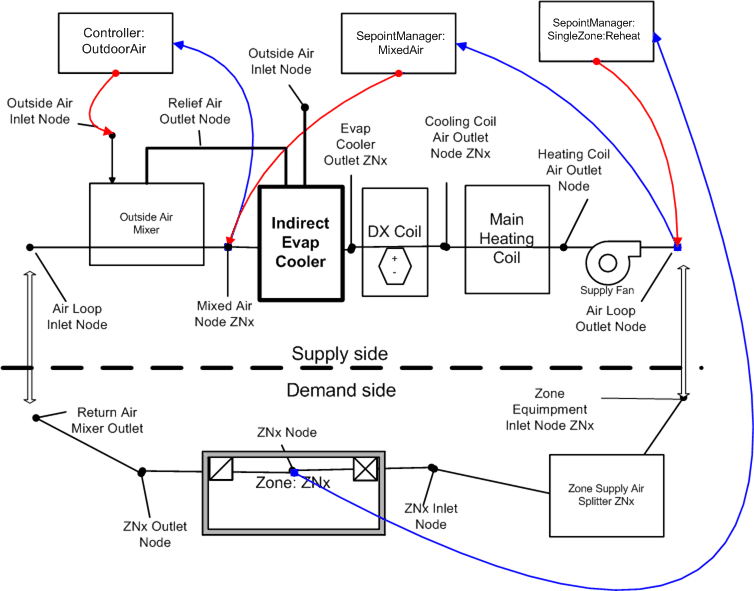
\includegraphics[width=0.9\textwidth, height=0.9\textheight, keepaspectratio=true]{media/image4833.png}
\caption{Research Special Indirect Evaporative Cooler Using Relief Air \protect \label{fig:research-special-indirect-evaporative-cooler-001}}
\end{figure}

\subsubsection{Indirect Evaporative Cooler Sizing}\label{indirect-evaporative-cooler-sizing-000}

The model for the object called EvaporativeCooler:Indirect:ResearchSpecial has a field for the secondary fan flow rate that can be autosized.

\paragraph{Secondary Air DesignFan Flow Rate}\label{secondary-air-designfan-flow-rate}

The secondary air design flow rate fan is not part of an airstream that is directly modeled in EnergyPlus. Because the primary side air flows can be autosized as part of the air system, it is convenentconvenient to also scale the size of the secondary flow. If the cooler is part of the main loop of a central air system, then the secondary fan flow rate is sized to equal to the main design flow rate.

User inputs for autosizing scaling factors are included so that when modeling an autosized IEC, all the design values can be scaled off of Primary Design Air Flow Rate. User input for Secondary Air Flow Sizing Factor is multiplied by DesMainVolFlow\(_{sys}\) as follows:

\begin{equation}
\dot{V}_{sec,design} = \text{DesMainVolFlow}_{sys}\cdot\text{SecAirFlowScalingFactor}
\end{equation}

If the cooler is part of the outdoor air path of a central air system, then the secondary air design flow rate is sized to be the maximum of either the design minimum outdoor air flow rate or one-half of the main design flow rate.

\begin{equation}
\dot{V}_{sec,design} = \max\left(\text{DesOutAirVolFlow},0.5\cdot\text{DesMainVolFlow}_{sys}\right)\cdot\text{SecAirFlowScalingFactor}
\end{equation}

\paragraph{Secondary Fan Design Power}\label{secondary-fan-design-power}

The Secondary Fan Design Power is outosized from secondary air design flow rate and user input for Secondary Fan Sizing Specific Power in units of W/(m3/s) as follows:

\begin{equation}
P_{sec,fan,design} = \dot{V}_{sec,design}\cdot\text{FanPowerScalingFactor}
\end{equation}

\paragraph{Recirculating Water Design Pump Power}\label{recirculating-water-design-pump-power}

The Recirculating Water Design Pump Power is sized from secondary air design flow rate and user input for recirculating and spraying Water Pump Power Sizing Factor in units of W/(m3/s) or W-s/m3 and is given by:

\begin{equation}
P_{pump,design} = \dot{V}_{sec,design}\cdot\text{PumpPowerScalingFactor}
\end{equation}

Where,

\(\dot{V}_{sys,design}\) = primary air design volume flow rate in m3/s

\(\dot{V}_{sec,design}\) = secondary air design volume flow rate in m3/s

\(\text{SecAirFlowScalingFactor}\) = user specified Secondary air flow sizing factor in units of W/(m3/s) for secondary design air flow rate calculation.

\(\text{FanPowerScalingFactor}\) = user specified secondary air fan sizing specific power in units of W/(m3/s) for design fan power calculation.

\(\text{PumpPowerScalingFactor}\) = user specified recirculating and spraying water pump power sizing factor in units of W/(m3/s) for design pump power calculation.

\subsection{Direct Evaporative Cooler Special Research Model}\label{direct-evaporative-cooler-special-research-model}

This section summarizes the model implemented in the component EvaporativeCooler:Direct:ResearchSpecial.~ This model can use a simple constant effectiveness or a variable effectiveness model that, under part load conditions, can modulate so that the air leaving the cooler just meets a drybulb temperature setpoint.~ The algorithm used to determine the changes to the system air proceeds in four steps:

\begin{enumerate}
\def\labelenumi{\arabic{enumi})}
\tightlist
\item
  Calculate the current operation effectiveness using effectiveness modifying curve
\end{enumerate}

2)~Calculate full load performance using a part load fraction (PLF) = 1 and Equation .

3)~Calculate PLF using Equations , , and .

4)~Recalculate cooler performance using the PLF.

\begin{equation}
 \begin{array}{rl}
  \epsilon_{op} & = \epsilon_{design}\cdot f_{mod}\left(flowRatio\right) \\
  T_{db,out,sys} & = T_{db,in,sys} - \epsilon_{op}\cdot\left(T_{db,in,sys}-T_{wb,in,sys}\right) \\
  T_{db,out} & = T_{db,in}-\epsilon\left(T_{db,in}-T_{wb,in}\right)
 \end{array}
\end{equation}

where,

\begin{itemize}
\item
  \({T_{db,out,sys}}\) ~is the drybub temperature of the air leaving the cooler {[}ºC{]},
\item
  \({T_{db,in,sys}}\) ~is the drybulb temperature of the air entering the cooler {[}ºC{]},
\item
  \({T_{wb,in,sys}}\) ~is the wetbulb temperature of the air entering the cooler {[}ºC{]}, and
\item
  \(\epsilon_{design}\) ~is the cooler design effectiveness.
\item
  \(\epsilon_{op}\) ~is the cooler current operation effectiveness.
\item
  \(f_{mod}\) ~is the effectiveness modifier curve as a function of system air flow fraction
\end{itemize}

The wetbulb temperature of air leaving a direct cooler is the same as the wetbulb temperature entering the cooler.~ The leaving humidity ratio of the air is calculated using psychrometric functions with leaving drybulb and wetbulb temperatures and outdoor air pressure as inputs.~ The leaving enthalpy of air is calculated using psychrometric functions with leaving drybulb temperature, leaving humidity ratio, and outdoor air pressure as inputs.

The direct cooler sometimes has the ability to overcool the air and therefore some form of modulation is useful for analysis.~ The special research model includes a Part Load Fraction, PLF, used to model the implications of controlling the amount of cooling.~ It is assumed that through some sort of on/off cycling or wetness control that the cooling electric power can be varied to exactly meet the desired temperature when PLF is less than unity.~ The auxiliary water pump power is then varied using pump power modifier curve or linearly using a Part Load Fraction when the pump power modifier curve is not specified.

\begin{equation}
{\rm{FullOutput}} = {T_{db,out}} - {T_{db,in}}
\end{equation}

\begin{equation}
{\rm{RequiredOutput}} = {T_{db,desired}} - {T_{db,in}}
\end{equation}

\begin{equation}
PLF = \frac{{{\rm{RequiredOutput}}}}{{{\rm{FullOutput}}}}
\end{equation}

When PLF is less than 1.0 it is assumed that the cooler will deliver the desired temperature air (as long as it is less than the inlet; it doesn't need heating).~ Water pump power is also derated using the user specified pump modifier curve or using PLF when the pump modifier curve is not specified.

\subsubsection{Water Consumption}\label{water-consumption-1}

Water consumption is an important consideration when evaluating evaporative coolers.~ Water consumption of the evaporative cooler is modeled using Equation .

\begin{equation}
{\dot V_{water}} = {\dot V_{evap}} + {\dot V_{drift}} + {\dot V_{blowdown}}
\end{equation}

The three components of water consumption are evaporation, drift, and blowdown.~ Evaporation is the water evaporated as the normal part of the evaporative cooler thermodynamic process and is calculated using:

\begin{equation}
{\dot V_{evap}} = \frac{{\dot m\left( {{w_{out}} - {w_{in}}} \right)}}{{{\rho_{water}}}}
\end{equation}

where,

\({\dot V_{evap}}\) ~is the volume flow rate of useful water evaporation {[}m\(^{3}\)/s{]}

\({w_{out}}\) ~is the humidity ratio of the air leaving the cooler {[}kg/kg{]}

\({w_{in}}\) ~is the humidity ratio of air entering the cooler {[}kg/kg{]}

\(\dot m\) ~is the mass flow rate of air moving through the cooler {[}kg/s{]}

\({\rho_{water}}\) ~is the density of water {[}kg/m3{]}

Drift is water that leaves the cooler (and supply air duct) as droplets and does not contribute to the evaporative cooling process in a useful manner.~ It is calculated using a user input factor that describes drift as a fraction of \({\dot V_{evap}}\) .

\begin{equation}
{\dot V_{drift}} = {\dot V_{evap}} * {f_{drift}}
\end{equation}

Blowdown is water drained from the sump to counter the build up of solids in the water that would otherwise occur because of evaporation.~ It is calculated using a user input factor for the blowdown concentration ratio ,\({R_{concentration}}\) , which is the ratio of solids in the blowdown water compared to the solids in the fresh makeup water and is limited to values of 2 or higher.~ The make up water needed for blowdown is calculated using:

\begin{equation}
{\dot V_{blowdown}} = \frac{{{{\dot V}_{evap}}}}{{\left( {{R_{concentration}} - 1.0} \right)}} - {\dot V_{drift}}
\end{equation}
